%%
%% 研究報告用スイッチ
%% [techrep]
%%
%% 欧文表記無しのスイッチ(etitle,eabstractは任意)
%% [noauthor]
%%

%\documentclass[submit,techrep]{ipsj}
\documentclass[submit,techrep,noauthor]{ipsj}


% \usepackage[dvips]{graphicx}
\usepackage[dvipdfmx, hiresbb]{graphicx}
\usepackage{latexsym}


\def\Underline{\setbox0\hbox\bgroup\let\\\endUnderline}
\def\endUnderline{\vphantom{y}\egroup\smash{\underline{\box0}}\\}
\def\|{\verb|}
%

%\setcounter{巻数}{59}%vol59=2018
%\setcounter{号数}{10}
%\setcounter{page}{1}


\begin{document}


\title{強化学習を用いたScratchにおける\\
リミックス元作品のCTスコア予測}

% \etitle{How to Prepare Your Paper for IPSJ SIG Technical Report \\ (version 2018/10/29)}

\affiliate{IPSJ}{情報処理学会\\
IPSJ, Chiyoda, Tokyo 101--0062, Japan}


\paffiliate{JU}{情報処理大学\\
Johoshori Uniersity}

\author{情報 太郎}{Joho Taro}{IPSJ}[joho.taro@ipsj.or.jp]
\author{処理 花子}{Shori Hanako}{IPSJ}
\author{学会 次郎}{Gakkai Jiro}{IPSJ,JU}[gakkai.jiro@ipsj.or.jp]

\begin{abstract}
本研究は,プログラミング初学者向けのビジュアルプログラミング言語Scratchにおいて,リミックス元作品のコンピュテーショナル・シンキング(CT)スコアを予測する手法を提案する.
従来研究では,他者の作品を複製・編集するリミックス機能が,学習者のCTスコア向上に有効であることが示されている.また,その効果はユーザの学習経験によって異なることが示唆された.しかし,現状ではユーザの学習経験に適したリミックス元作品を見つけることが困難である.
本研究では,Scratchに参加するユーザが作品制作した過程をマルコフ決定過程として捉え,強化学習を用いてユーザが選択するリミックス元作品のCTスコアを予測するモデルを構築する.これにより,ユーザの過去作品やリミックス履歴に基づいたCTスコアの推定が可能となり,今後のリミックス元作品の選択の指針となることを目指す.
\end{abstract}


%
%\begin{jkeyword}
%情報処理学会論文誌ジャーナル,\LaTeX,スタイルファイル,べからず集
%\end{jkeyword}
%
%\begin{eabstract}
%This document is a guide to prepare a draft for submitting to IPSJ
%Journal, and the final camera-ready manuscript of a paper to appear in
%IPSJ Journal, using {\LaTeX} and special style files.  Since this
%document itself is produced with the style files, it will help you to
%refer its source file which is distributed with the style files.
%\end{eabstract}
%
%\begin{ekeyword}
%IPSJ Journal, \LaTeX, style files, ``Dos and Dont's'' list
%\end{ekeyword}

\maketitle

%1
\section{はじめに}

近年,日本では2020年度から小学校のプログラミング教育の必修化,2021年度から中学校の技術分野において,プログラミングに関する内容の充実,2022年度から高等学校の情報科において,共通必履修科目「情報1」の新設がされている\cite{monkashou}.しかし,指導者の情報不足や人材不足,予算不足による指導者に対する問題が複数挙げられた\cite{monkashou2}.以前からプログラミング教育に力を注いでいるアメリカでは,Scratch\footnote{https://scratch.mit.edu/}\cite{resnick2009scratch}と呼ばれるプログラミング初学者向けのビジュアルプログラミング言語を通してプログラミング教育を行っている.Scratchでは「繰り返す」などの命令処理をもつブロックを,ジグソーパズルのように組み合せることで作品を完成させる.さらに,完成した作品はオンライン上に公開することができ,公開されている他ユーザの作品は,見る,使うだけでなく,複製し,編集することも可能である.この機能はリミックスと呼ばれる.

ビジュアルプログラミングは,プログラミング初学者が取り組みやすいような環境にするとともに,コンピュテーショナル・シンキング(CT)\cite{wing2006computational}スキルの向上を目的としている.学習や操作のハードルが低いため,プログラミングの入門学習として有効である.また,バグが少なく,直観的な操作のみでプログラミングをすることができるため,ユーザが短期間で作品を完成させやすく,達成感を得やすいという特徴をもつ.近年では,情報化社会の進展に伴い,プログラマー不足が深刻な問題となっている.ビジュアルプログラミング言語の活用はその課題解決の第一歩になると考えられる.

CTスキルを自身で評価・把握することは困難である.そのため,Morenoらは作品に使用されているブロックに基づき,CTスキルを計測するDr.Scratch\cite{moreno2015dr}を開発した.Dr.Scratchでは,論理,制御フロー,同期,抽象化,データ表現,ユーザ対話性,並列処理の7概念に基づいて作品評価を行う.また,各概念を0点から3点の合計21点とし,CTスコアとして評価する.表\ref{CTscoreTable}に各概念の評価方法を示す.CTスコアを3つの区分に分類し,0点から7点をBasic,8点から14点をDeveloping,15点から21点をMasterとして評価する.

\begin{table*}[t] % table環境をtable*に変更
    \centering
    \caption{CTスコア概念\cite{hashitani2022scratch}}
    \label{CTscoreTable}
    % table*はページ全体を使うため、scaleboxを調整するか、削除を検討。
    % ページ幅全体に広げるため、0.55から0.8~0.9などに広げても良いでしょう。
    \scalebox{0.8}{ % ページ幅全体を使うため、スケールを0.8などに広げました
    \begin{tabular}{c|c|c|c|c}
    \hline
    CTスキルの概念 & 0点 & 1点 & 2点 & 3点
    \\ \hline
    抽象化 & - &
    \begin{tabular}{c}
    2つ以上の\\スクリプトを使用
    \end{tabular}
    & 定義ブロックを使用 & クローンブロックを使用
    \\ \hline
    並列 & - & 
    \begin{tabular}{c}
    緑の旗ブロックを\\2個以上使用 
    \end{tabular}
    & 
    \begin{tabular}{c}
    オブジェクトへのクリックにより\\2つ以上のスクリプトを\\同時に実行する機能を実装
    \end{tabular}
    & 
    \begin{tabular}{c}
    イベント動作により\\2つ以上のスクリプトを\\同時に実行する機能を実装
    \end{tabular}
    \\ \hline
    論理 & - & Ifブロックを使用 & If elseブロックを使用 & 論理演算ブロックを使用
    \\ \hline
    同期 & - & 待機ブロックを使用 &
    \begin{tabular}{c}
    メッセージ受信により\\プログラムを停止する機能を実装
    \end{tabular}
    &
    \begin{tabular}{c}
    指定条件を満たすまで\\プログラムを停止する処理を実装
    \end{tabular}
    \\ \hline
    フロー制御 & - &
    \begin{tabular}{c}
    2個以上の処理ブロックを\\連結して使用
    \end{tabular}
    &
    \begin{tabular}{c}
    指定回数/回数無制限の\\繰り返しブロックを使用
    \end{tabular}
    &
    \begin{tabular}{c}
    指定条件までの\\繰り返しブロックを使用
    \end{tabular}
    \\ \hline
    ユーザ対話性 & - & 緑の旗ブロックを使用 &
    \begin{tabular}{c}
    ユーザの入力を伴う\\ブロックを使用
    \end{tabular}
    &
    \begin{tabular}{c}
    マイクやビデオなどの\\作用を伴うブロックを使用
    \end{tabular}
    \\ \hline
    データ表現 & - &
    \begin{tabular}{c}
    オブジェクトの\\プロパティを編集
    \end{tabular}
    & 変数ブロックを使用 & リスト変数ブロックを使用
    \\ \hline
    \end{tabular}
    }
\end{table*}

\begin{itemize}
  \item 状態
    
    $s_t$:ある作品制作地点での状態(8次元)

    $x_t$:ある作品のCTスコア概念のベクトル(7次元)

    $m_t\in\{0,1\}$:リミックスであるか否か(1次元)

    \begin{equation}
        s_t = 
        \begin{bmatrix}
           x_t \\
           m_t 
        \end{bmatrix}
    \end{equation}

  \item 行動

    $a_t$:選択したリミックス元作品のCTスコア概念のベクトル(7次元)

    % $a_t$:t+1番目に制作する作品のCTスコア概念のベクトル(7次元)
  
  \item 報酬

    $r_t$:リミックス前後作品のCTスコアの差分のスカラー
    
    $c_t$:リミックス前作品のCTスコア

    $c'_t$:リミックス後作品のCTスコア
    
    \begin{equation}
        r_t = c'_t - c_t
    \end{equation}

    % $r_t$:前後作品のCTスコアの差分のスカラー
    
    % $c_t$:t番目の作品のCTスコア

    % $c'_t$:t-1番目の作品のCTスコア
    
    % \begin{equation}
    %     r_t = c'_t - c_t
    % \end{equation}
  
  \item 状態遷移確率:
\end{itemize}

\section{RQ1}

図\ref{heatmap}が示すように

\begin{figure*}[t]
  \centering
  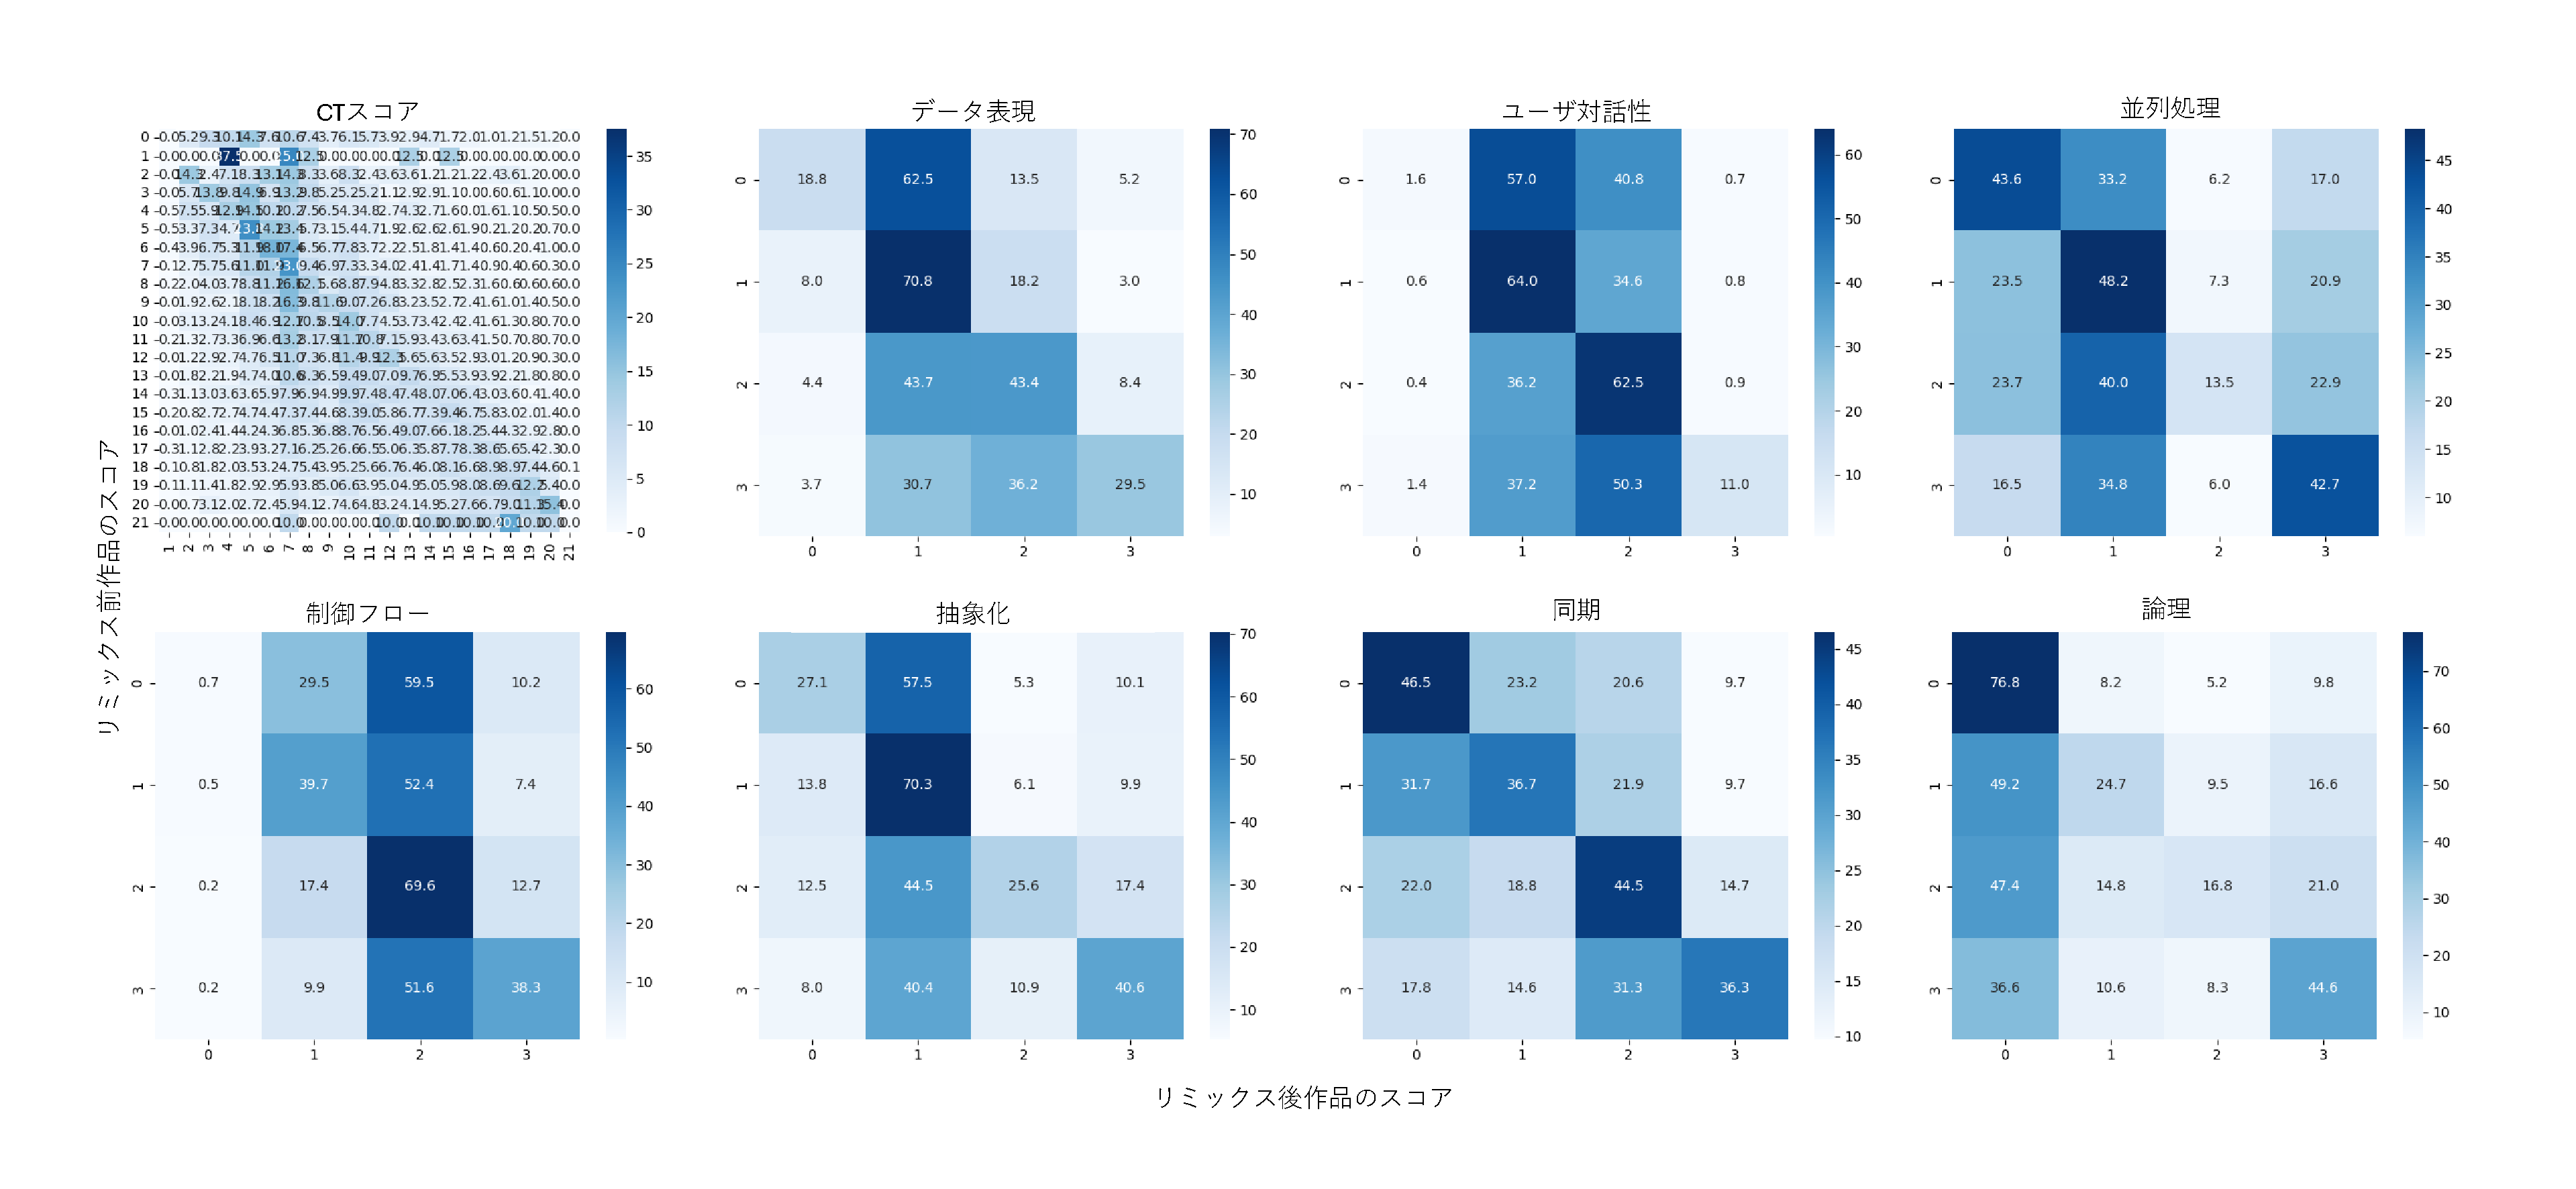
\includegraphics[width=\textwidth]{@IPSJ_SIGSE202511_Horio/heatmap.pdf}
  \caption{ヒートマップ}
  \label{heatmap}
\end{figure*}

% %2
% \section{投稿の流れ}

% %2.1
% \subsection{準備}

% 情報処理学会論文誌ジャーナルの\LaTeX スタイルファイルを含む論文執筆キットは
% \begin{quote}
% \small
% \|http://www.ipsj.or.jp/jip/submit/style.html|
% \end{quote}
% からダウンロードすることができる.論文執筆キットは以下のファイルを含んで
% いる.
% \begin{enumerate}
% \item \|ipsj.cls      |: 最終原稿用スタイルファイル
% \item \|ipsjdraft.sty |: 投稿用スタイル(査読用)
% \item \|ipsjpref.sty  |: 序文用スタイル
% \item \|jsample.tex   |: 本稿のソースファイル
% \item \|esample.tex   |: 英文サンプルのソースファイル
% \item \|ipsjsort.bst  |: jBibTEX スタイル(著者名順)
% \item \|ipsjunsrt.bst |: jBibTEX スタイル(出現順)
% \item \|bibsample.bib |: 文献リストのサンプル
% \item \|ebibsample.bib|: 英文文献リストのサンプル
% \item \|tech-jsample.tex:| 研究報告(和文)のサンプル
% \item \|tech-esample.tex:| 研究報告(英文)のサンプル
% \end{enumerate}
% 実行環境としては\LaTeXe を前提としているので,準備されたい.

%2.2
% \subsection{原稿の作成と投稿}

% 本稿に従って用意した投稿用原稿の\LaTeX ソースからpdfファイルを作成し,
% Adobeのpdf readerで読めることを確認した後,
% \begin{quote}
% \small
% \|https://ipsj1.i-product.biz/ipsjsig/**|
% \end{quote}
% (**部分は研究会の略称,DBS等)の研究会投稿システムにて,指示にし従い投稿する.







%3
% \section{論文フォーマットの指針}
% \label{sec:format}

% 以下,情報処理学会論文誌ジャーナル用スタイルファイルを用いた論文フォーマットの指針について述べるので,
% これに従って原稿を用意頂きたい.
% \LaTeX を用いた一般的な文章作成技術については,
% \cite{okumura, companion} 等を参考にされたい.



% %4
% \section{論文の構成}
% \label{config}

% ファイルは次のようになる.下線部は投稿時に省略可能なもの.

% \noindent
% \|\documentclass[submit,techrep,noauthor]{ipsj}|\\
% \quad 必要ならばユーザのマクロをここに記述\\
% \|\begin{document}|\\
% \|\title{表題(和文)}|\\
% \|\etitle{表題(英文)}|\\
% \Underline{\|\affiliate{所属ラベル}{<和文所属>\\<英文所属>}|}\\
% \quad 必要ならば \|\paffiliate| により現在の所属を宣言する\\
% \Underline{\|\paffiliate{現所属ラベル}{<和現所属>\\<英現所属>}|}\\\\
% \Underline{\|\author{情報 太郎}{Taro Joho}|}\\
% \Underline{\|          {<所属ラベル>}[E-mail]|}\\
% \Underline{\|\author{処理 花子}{Hanako Shori}|}\\
% \Underline{\|          {<所属ラベル2,現所属ラベル3>}|}\\\\
% \|\begin{abstract}|\\
% \|<概要(和文)>|\\
% \|\end{abstract}|\\
% \|\begin{eabstract}|\\
% \|<概要(英文)>|\\
% \|\end{eabstract}|\\
% \|\maketitle|\\
% \|\section{|第1節の表題\|}|\\
% \dots\dots\dots\dots\dots\\
% \quad \|<本文>|\\
% \dots\dots\dots\dots\dots\\
% 謝辞がある場合は\\
% \|\begin{acknowledgment}|\\
% \|\end{acknowledgment}|\\\\
% \|\begin{thebibliography}{99}%9 or 99|\\
% \|\bibitem{1}|\\
% \|\bibitem{2}|\\
% \|\end{thebibliography}|\\\\
% 付録がある場合は\\
% \|\appendix|\\
% \|\section{|付録1節の表題\|}|\\
% \|\end{document}|




%4.1
% \subsection{表題・著者名等}

% 表題,著者名とその所属,および概要を前述のコマンドや環境により{\bf 和文と
% 英文の双方について}定義した後,\|\maketitle| によって出力する.


% \newpage%%%%%

%4.1.1
% \subsubsection{表題} 

% 表題は,\|\title| および \|\etitle| で定義した表題はセンタリングされる.
% 文字数の多いものについては,適宜 \|\\| を挿入して改行する.

%4.1.2
% \subsubsection{著者名・所属} 

% 各著者の所属を第一著者から順に \|\affiliate| を用いてラベル(第1引数)を付けながら定義すると,
% 脚注に番号を付けて所属が出力される.
% なお,複数の著者が同じ所属である場合には,
% 一度定義するだけで良い.



% 現在の所属は \|\paffiliate| を用い,同様にラベル,所属先を記述する.
% 所属先には自動で「現在」,
% \|\\|の改行で「Presently with」が挿入される.
% 著者名は \|\author| で定義する.各著者名の直後に,英文著者名,
% 所属ラベルとメールアドレスを記入する.
% 著者が複数の場合は \|\author| を繰り返すことで,
% 2人,3人,\dots と増えていく.
% 現在の所属や,複数の所属先を追加する場合には,所属ラベルをカンマで区切り,追加すればよい.


% また,メールアドレス部分は省略が可能である.





%4.1.3
% \subsubsection{概要} 

% 和文の概要は \|abstract| 環境の中に,
% 英文の概要は \|eabstract| 環境の中に,それぞれ記述する.



%4.2
% \subsection{本文}

%4.2.1
% \subsubsection{見出し}

% 節や小節の見出しには \|\section|, \|\subsection|, \|\subsubsection|,
% \|\paragraph| といったコマンドを使用する.

% \<「定義」,「定理」などについては,\|\newtheorem|で適宜環境を宣言し,そ
% の環境を用いて記述する.

%4.2.2
% \subsubsection{行送り}

% 2段組を採用しており,左右の段で行の基準線の位置が一致することを原則としている.
% また,節見出しなど,
% 行の間隔を他よりたくさんとった方が読みやすい場所では,
% この原則を守るようにスタイルファイルが自動的にスペースを挿入する.
% したがって本文中では \|\vspace| や \|\vskip| を用いたスペースの調整を行なわないようにすること.


%4.2.3
% \subsubsection{フォントサイズ}

% フォントサイズは,スタイルファイルによって自動的に設定されるため,
% 基本的には著者が自分でフォントサイズを変更する必要はない.

%4.2.4
% \subsubsection{句読点}

% 句点には全角の「.」,
% 読点には全角の「,」を用いる.
% ただし英文中や数式中で「.」や「,」を使う場合には,
% 半角文字を使う.「。」や「、」は使わない.



%4.2.5
% \subsubsection{全角文字と半角文字}

% 全角文字と半角文字の両方にある文字は次のように使い分ける.

% \begin{enumerate}
% \item 括弧は全角の「(」と「)」を用いる.但し,英文の概要,図表見出し,
% 書誌データでは半角の「(」と「)」を用いる.

% \item 英数字,空白,記号類は半角文字を用いる.ただし,句読点に関しては,
% 前項で述べたような例外がある.

% \item カタカナは全角文字を用いる.

% \item 引用符では開きと閉じを区別する.
% 開きには \|``| を用い,閉じには\|''| を用いる.
% \end{enumerate}

%4.2.6
% \subsubsection{箇条書}

% 箇条書に関する形式を特に定めていない.場合に応じて標準的な \|enumerate|,
% \|itemize|, \|description| の環境を用いてよい.


%4.2.7
% \subsubsection{脚注}

% 脚注は \|\footnote| コマンドを使って書くと,
% ページ単位に\footnote{脚注の例.}や\footnote{二つめの脚注.}のような参照記号とともに脚注が生成される.
% なお,ページ内に複数の脚注がある場合,参照記号は\LaTeX を2回実行しないと正しくならないことに注意されたい.



% また場合によっては,
% 脚注をつけた位置と脚注本体とを別の段に置く方がよいこともある.
% この場合には,\|\footnotemark| コマンドや \|\footnotetext| コマンドを使って対処していただきたい.


% なお,脚注番号は論文内で通し番号で出力される.




%4.2.8
% \subsubsection{OverfullとUnderfull}

% 組版時にはoverfullを起こさないことを原則としている.
% 従って,まず提出するソースが著者の環境でoverfullを起こさないように,
% 文章を工夫するなどの最善の努力を払っていただきたい.
% 但し,\|flushleft| 環境,\|\\|,\|\linebreak| などによる両端揃えをしない形でのoverfullの回避は,
% できるだけ避けていただきたい.
% また著者の執筆時点では発生しないoverfullが,
% 組版時の環境では発生することもある.
% このような事態をできるだけ回避するために,
% 文中の長い数式や \|\verb| を避ける,
% パラグラフの先頭付近では長い英単語を使用しない,
% などの注意を払うようにして頂きたい.




%4.3
% \subsection{数式}\label{sec:Item}

%4.3.1
% \subsubsection{本文中の数式}

% 本文中の数式は \|$| と \|$|, \|\(| と \|\)|, あるいは \|math| 環境のいず
% れで囲んでもよい.

%4.3.2
% \subsubsection{別組の数式}

% 別組数式(displayed math)については \|$$| と \|$$| は使用せずに,
% \|\[| と \|\]| で囲むか,
% \|displaymath|, \|equation|, \|eqnarray| のいずれかの環境を用いる.
% これらは
% %
% \begin{equation}
% \Delta_l = \sum_{i=l|1}^L\delta_{pi}
% \end{equation}
% %
% のように,センタリングではなく固定字下げで数式を出力し,
% かつ背が高い数式による行送りの乱れを吸収する機能がある.

%4.3.3
% \subsubsection{eqnarray環境}

% 互いに関連する別組の数式が2行以上連続して現れる場合には,
% 単に\|\[| と \|\]|,
% あるいは \|\begin{equation}| と\|\end{equation}| で囲った数式を書き並べるのではなく,
% \|\begin|\allowbreak\|{eqnarray}| と \|\end{eqnarray}| を使って,
% 等号(あるいは不等号)の位置で縦揃えを行なった方が読みやすい.


%4.3.4
% \subsubsection{数式のフォント}

% \LaTeX が標準的にサポートしているもの以外の特殊な数式用フォントは,
% できるだけ使わないようにされたい.
% どうしても使用しなければならない場合には,
% その旨申し出て頂くとともに,
% 組版工程に深く関与して頂くこともあることに留意されたい.


% \begin{figure}[tb]
% \setbox0\vbox{
% \hbox{\|\begin{figure}[tb]|}
% \hbox{\quad \|<|図本体の指定\|>|}
% \hbox{\|\caption{<|和文見出し\|>}|}
% \hbox{\|\ecaption{<|英文見出し\|>}|}
% \hbox{\|\label{| $\ldots$ \|}|}
% \hbox{\|\end{figure}|}
% }
% \centerline{\fbox{\box0}}
% \caption{1段幅の図}
% \ecaption{Single column figure with caption\\
% explicitly broken by $\backslash\backslash$.}
% \label{fig:single}
% \end{figure}



%4.4
% \subsection{図}

% 1段の幅におさまる図は,
% \figref{fig:single} の形式で指定する.
% 位置の指定に \|h| は使わない.
% また,図の下に和文と英文の双方の見出しを,
% \|\caption| と \|\ecaption| で指定する.
% 文字数が多い見出しはは自動的に改行して最大幅の行を基準にセンタリングするが,
% 見出しが2行になる場合には適宜 \|\\| を挿入して改行したほうが良い結果となることがしばしばある
% (\figref{fig:single} の英文見出しを参照).
% 図の参照は \|\figref{<|ラベル\|>}| を用いて行なう.




% \begin{figure}[tb]
% \begin{minipage}[t]{0.5\columnwidth}
% \footnotesize
% \setbox0\vbox{
% \hbox{\|\begin{minipage}[t]%|}
% \hbox{\|  {0.5\columnwidth}|}
% \hbox{\|\CaptionType{table}|}
% \hbox{\|\caption{| \ldots \|}|}
% \hbox{\|\ecaption{| \ldots \|}|}
% \hbox{\|\label{| \ldots \|}|}
% \hbox{\|\makebox[\textwidth][c]{%|}
% \hbox{\|\begin{tabular}[t]{lcr}|}
% \hbox{\|\hline\hline|}
% \hbox{\|left&center&right\\\hline|}
% \hbox{\|L1&C1&R1\\|}
% \hbox{\|L2&C2&R2\\\hline|}
% \hbox{\|\end{tabular}}|}
% \hbox{\|\end{minipage}|}}
% \hbox{}
% \centerline{\fbox{\box0}}
% \caption{\protect\tabref*{tab:right} の中身}
% \ecaption{Contents of Table \protect\ref{tab:right}.}
% \label{fig:left}
% \end{minipage}%
% \begin{minipage}[t]{0.5\columnwidth}
% \CaptionType{table}
% \caption{\protect\figref*{fig:left} で作成した表}
% \ecaption{A table built by\\ Fig.\,\protect\ref{fig:left}.}
% \label{tab:right}
% \vskip1mm
% \makebox[\textwidth][c]{\begin{tabular}[t]{lcr}\hline\hline
% left&center&right\\\hline
% L1&C1&R1\\
% L2&C2&R2\\\hline
% \end{tabular}}
% \end{minipage}
% \end{figure}

% \begin{figure*}[tb]
% \setbox0\vbox{\large
% \hbox{\|\begin{figure*}[t]|}
% \hbox{\quad \|<|図本体の指定\|>|}
% \hbox{\|\caption{<|和文見出し\|>}|}
% \hbox{\|\ecaption{<|英文見出し\|>}|}
% \hbox{\|\label{| $\ldots$ \|}|}
% \hbox{\|\end{figure*}|}}
% \centerline{\fbox{\hbox to.9\textwidth{\hss\box0\hss}}}
% \caption{2段幅の図}
% \ecaption{Double column figure.}
% \label{fig:double}
% \end{figure*}


% また紙面スペースの節約のために,
% 1つの \|figure|(または \|table|)環境の中に複数の図表を並べて表示したい場合には,
% \figref{fig:left} と \tabref{tab:right} のように個々の図表と各々の \|\caption|/\|\ecaption| 
% を \|minipage| 環境に入れることで実現できる.
% なお図と表が混在する場合,
% \|minipage| 環境の中で\|\CaptionType{figure}| あるいは \|\CaptionType|
% \|{table}| を指定すれば,
% 外側の環境が \|figure| であっても \|table| であっても指定された見出しが得られる.



% 2段の幅にまたがる図は,
% \figref{fig:double} の形式で指定する.
% 位置の指定は \|t| しか使えない.



% 図の中身では本文と違い,
% どのような大きさのフォントを使用しても構わない(\figref{fig:double} 参照).
% また図の中身として,encapsulate されたPostScriptファイル(いわゆるEPSファイル)を読み込むこともできる.
% 読み込みのためには,プリアンブルで
% %
% \begin{quote}
% \|\usepackage{graphicx}|
% \end{quote}
% %
% を行った上で,
% \|\includegraphics| コマンドを図を埋め込む箇所に置き,
% その引数にファイル名(など)を指定する.




%4.5
% \subsection{表}

% 表の罫線はなるべく少なくするのが,仕上がりをすっきりさせるコツである.
% 罫線をつける場合には,
% 一番上の罫線には二重線を使い,左右の端には縦の罫線をつけない (\tabref{tab:example}).
% 表中のフォントサイズのデフォルトは\|\footnotesize|である.


% また,表の上に和文と英文の双方の見出しを,
% \|\caption|と \|\ecaption| で指定する.
% 表の参照は \|\tabref{<|ラベル\|>}| を用いて行なう.

% \begin{table}[tb] 
% \caption{表の例} 
% \ecaption{An Example of Table.}
% \label{tab:example}
% \hbox to\hsize{\hfil
% \begin{tabular}{l|lll}\hline\hline
% & column1 & column2 & column3 \\\hline
% row1 &	item 1,1 & item 2,1 & ---\\
% row2 &	---      & item 2,2 & item 3,2 \\
% row3 &	item 1,3 & item 2,3 & item 3,3 \\
% row4 &	item 1,4 & item 2,4 & item 3,4 \\\hline
% \end{tabular}\hfil}
% \end{table}




% \newpage%%%%%

%4.6
% \subsection{参考文献・謝辞}

% %4.6.1
% \subsubsection{参考文献の参照}

% 本文中で参考文献を参照する場合には\|\cite|を使用する.
% 参照されたラベルは自動的にソートされ,
% \|[]|でそれぞれ区切られる.
% %
% \begin{quote}
% 文献 \|\cite{companion,okumura}| は\LaTeX の総合的な解説書である.
% \end{quote}
% %
% と書くと;
% %
% \begin{quote}
% 文献\cite{companion,okumura}は\LaTeX の総合的な解説書である.
% \end{quote}
% %
% が得られる.

% %4.6.2
% \subsubsection{参考文献リスト}
% 参考文献リストには,
% 原則として本文中で引用した文献のみを列挙する.
% 順序は参照順あるいは第一著者の苗字のアルファベット順とする.
% 文献リストはBiB\TeX と\verb+ipsjunsrt.bst+(参照順)
% または\verb+ipsjsort.bst+(アルファベット順)を用いて作り,
% \verb+\bibliograhpystyle+と\verb+\bibliography+コマンドにより
% 利用することが出来る.
% これらを用いれば,
% 規定の体裁にあったものができるので,
% できるだけ利用していただきたい.
% また製版用のファイル群には\verb+.bib+ファイルではなく\verb+.bbl+ファイルを
% 必ず含めることに注意されたい.
% 一方,何らかの理由でthebibliography環境で文献リストを
% 「手作り」しなければならない場合は,
% このガイドの参考文献リストを注意深く見て,
% そのスタイルにしたがっていただきたい.




% %4.6.3
% \subsubsection{謝辞}

% 謝辞がある場合には,
% 参考文献リストの直前に置き,
% \|acknowledgment|環境の中に入れる.



% %5
% \section{論文内容に関する指針}

% 論文の内容について,
% 論文誌ジャーナル編集委員会で作成した「べからず集」を以下に示す.
% 投稿前のチェックリストとして利用頂きたい.
% これ以外にも,査読者用,
% メタ査読者用の「べからず集」\cite{webpage2}も公開しているので,
% 参照されたい.
% また,作文技術に関する \cite{book1, book2, book3, book4}のような書籍も参考になる.



% %5.1
% \subsection{書き方の基本}

% \begin{itemize}
%  \item[$\Box$] 研究の新規性,有用性,信頼性が読者に伝わるように記述する.
%  \item[$\Box$] 読み手に,読みやすい文章を心がける(内容が前後する,背景・
% 	       課題の設定が不明瞭などは読者にとって負担).
%  \item[$\Box$] 解決すべき問題が汎用化(一般的に記述)されていないのは再
% 	       考を要する(XX大学の問題という記述に終始).あるいは,
% 	       (単に「作りました」だけで)解決すべき問題そのものの記述
% 	       がないのは再考を要する.
%  \item[$\Box$] 結論が明確に記されていない,または,範囲,限界,問題点な
% 	       どの指摘が適切ではない,または,結論が内容にそったもので
% 	       はないものは再考を要する.
%  \item[$\Box$] 科学技術論文として不適当な表現や,分かりにくい表現がある
% 	       のは再考を要する.
%  \item[$\Box$] 極端な口語体や,長文の連続などは再考を要する.
%  \item[$\Box$] 章,節のたて方,全体の構成等が適切でない文章は再考を要す
% 	       る.
%  \item[$\Box$] 文中の文脈から推測しないと内容の把握が困難な論文にしない.
%  \item[$\Box$] 説明に飛躍した点があり,仮説等の説明が十分ではないのは再
% 	       考を要する.
%  \item[$\Box$] 説明に冗長な点,逆に簡単すぎる点があるのは再考を要する.
%  \item[$\Box$] 未定義語を減らす.
% \end{itemize}


% %5.2
% \subsection{新規性と有効性を明確に示す}

% \begin{itemize}
%  \item[$\Box$] 在来研究との関連,研究の動機,ねらい等が明確に説明されて
% 	       いないのは再考を要する.
%  \item[$\Box$] 既知/公知の技術が何であって,何を新しいアイデアとして提
% 	       案しているのかが書かれていないのは再考を要する.
%  \item[$\Box$] 十分な参考文献は新規性の主張に欠かせない.
%  \item[$\Box$] 提案内容の説明が,概念的または抽象的な水準に終始していて,
% 	       読者が提案内容を理解できない(それだけで新規性が感じられ
% 	       ないもの)のは再考を要する.
%  \item[$\Box$] 論文で提案した方法の有効性の主張がない,またはきわめて貧
% 	       弱なのは再考を要する.
% \end{itemize}

% %5.3
% \subsection{書き方に関する具体的な注意}

% \begin{itemize}
%  \item[$\Box$] 和文標題が内容を適切に表現していないのは再考を要する.
%  \item[$\Box$] 英文標題が内容を適切に表現していない,または英語として適
% 	       切でないのは再考を要する.
%  \item[$\Box$] アブストラクトが主旨を適切に表現していない,または英文が
% 	       適切ではないのは再考を要する.
%  \item[$\Box$] 記号・略号等が周知のものでなく,または,用語が適切でなく,
% 	       または,図・表の説明が適当ではないのは再考を要する.
%  \item[$\Box$] 個人的あるいは非常に小さなグループ/企業だけで通用するよ
% 	       うな用語が特別な説明もなしに多用されているのは再考を要す
% 	       る.
%  \item[$\Box$] 図表自体は十分に明確ではない,または誤りがあるのは再考を
% 	       要する.
%  \item[$\Box$] 図表が鮮明ではないのは再考を要する.
%  \item[$\Box$] 図表が大きさ,縮尺の指定が適切でないのは再考を要する.
% \end{itemize}

% %5.4
% \subsection{参考文献}

% \begin{itemize}
%  \item[$\Box$] 参考文献は10件以上必要(分野によっては20件以上,30件以上
% 	       という意見もある).
%  \item[$\Box$] 十分な参考文献は新規性の主張に欠かせない.
%  \item[$\Box$] 適切な文献が引用されておらず,その数も適切ではないのは再
% 	       考を要する.
%  \item[$\Box$] 日本人によるしかるべき論文を引用することで日本人研究コミュ
% 	       ニティの発展につながる.
%  \item[$\Box$] 参考文献は自分のものばかりではだめ.
% \end{itemize}

% %5.5
% \subsection{二重投稿}

% \begin{itemize}
%  \item[$\Box$] 二重投稿はしてはならない ─ ただし国際会議に採択された論
% 	       文を著作権が問題にならないように投稿することは構わない.
%  \item[$\Box$] 他の論文とまったく同じ図表を引用の明示なしに利用すること
% 	       は禁止.
%  \item[$\Box$] 既発表の論文等との間に重複があるのは再考を要する.
% \end{itemize}

% %5.6
% \subsection{他の人に読んでもらう}

% \begin{itemize}
%  \item[$\Box$] 投稿経験が少ない人は,採録された経験の豊富な人に校正して
% 	       もらう.
%  \item[$\Box$] 読者の立場から見て論理的な飛躍がないかに注意して記述する.
% \end{itemize}

% %5.7
% \subsection{その他}

% \begin{itemize}
%  \item[$\Box$] 投稿前にチェックリストの各項目を満たしているか,必ず確認
% 	       する. 
% \end{itemize}

% %6
% \section{おわりに}

% 本稿では,A4縦型2段組み用に変更したスタイルファイルを用いた論文のフォー
% マット方法と,論文誌ジャーナル編集委員会がまとめた「べからず集」に基づく
% 論文の書き方を示した.内容的にまだ不十分の部分が多いため,意見,要望等を
% \begin{quote}
%  \|editt@ipsj.or.jp|
% \end{quote}
% までお寄せ頂きたい.



% \begin{acknowledgment}
% A4横型に対するガイドを基に,本稿を作成した.
% クラスファイルの作成においては,
% 京都大学の中島 浩氏にさまざまなご教示を頂き,
% さらにBiB\TeX 関連ファイルの利用についても快諾頂いたことを深謝する.
% また,A4横型に対するガイドを作成された当時の編集委員会の担当者に深謝する.
% \end{acknowledgment}



% \begin{thebibliography}{10}

% \bibitem{okumura}
% 奥村晴彦:改訂第5版\LaTeXe 美文書作成入門,
% 技術評論社(2010).

% \bibitem{companion}
% Goossens, M., Mittelbach, F. and Samarin, A.:
% {\it The LaTeX Companion},
% Addison Wesley, Reading, Massachusetts (1993).

% \bibitem{book1}
% 木下是雄:
% 理科系の作文技術,
% 中公新書(1981).

% \bibitem{book2}
% Strunk W. J. and White E.B.:
% {\it The Elements of Style, Forth Edition},
% Longman (2000).

% \bibitem{book3}
% Blake G. and Bly R.W.:
% {\it The Elements of Technical Writing},
% Longman (1993).

% \bibitem{book4}
% Higham N.J.:
% {\it Handbook of Writing for the Mathematical Sciences},
% SIAM (1998).

% \bibitem{webpage1}
% 情報処理学会論文誌ジャーナル編集委員会:
% 投稿者マニュアル(online),
% \urlj{http://www.ipsj.or.jp/journal /submit/manual/j\_manual.html}
% (2007.04.05).

% \bibitem{webpage2}
% 情報処理学会論文誌ジャーナル編集委員会:
% べからず集(online),
% \urlj{http://www.ipsj.or.jp/journal/manual /bekarazu.html}
% (2011.09.15).

% \end{thebibliography}

\bibliographystyle{unsrt}
\bibliography{references}

\end{document}
